\documentclass{beamer}

\usepackage{graphicx}
\usepackage{amsmath}
\usepackage{amsthm}

\theoremstyle{definition}
% 'definition' environment is already defined by the beamer class; do not redefine it.
% \newtheorem{definition}{Definition}

% \theoremstyle{plain}
% \newtheorem{theorem}{Theorem}

\theoremstyle{remark}
\newtheorem{remark}{Remark}

\title{Week 6 CUSF Output Feedback 1: }
\author{Yoonjae Hwang}
\date{16 November 2025}

\begin{document}
\frame{\titlepage}

\begin{frame}
\frametitle{Motivation}
A system can only estimate what it is doing and where it is using it's sensors.
We need to be able to use sensor information to infer what the system is doing. 
This process is called observer design. 
We never actually have access to the true "state". We can only use the estimated "state". 
\newline
Sensors are also prone to noise, and disturbances. How do we deal with this?  
\end{frame}

\begin{frame}
\frametitle{Observability}
\begin{definition}[Observability]
A linear system is \textsl{observable} if for every $T > 0$ it is 
possible to determine the state of the system $x(T)$ from measurements 
of $y(t)$ and $u(t)$ on the interval $[0, T]$.
\end{definition}
The idea is, we want to know if we can deduce what the state is by looking at the measured values. 
\end{frame}

\begin{frame}
\frametitle{Observability}
Observability is not about driving the system, but rather watching it. 
So let us consider an autonomous system: 
\begin{equation}
    \dot{x} = A x \qquad y =  C x
\end{equation}
We can easily write the explicit solution for this: 
\begin{equation}
    x(t) = e^{At} x_0 \qquad y(t) = Ce^{At}x_0
\end{equation}
where $x_0 = x(0)$.
At time $t=T$, the state and output will be: 
\begin{equation}
    x(T) = e^{AT} x_0 \qquad y(T) = Ce^{AT}x_0
\end{equation}
\end{frame}

\begin{frame}
\frametitle{Observability}
Now we consider sufficiently many time derivatives to form a system of linear equations:
\begin{equation}
\begin{aligned}
y(T) &= Ce^{AT}x_0 \\ 
\dot{y}(T) &= CAe^{AT}x_0 \\
\ddot{y}(T) &= CA^2 e^{AT}x_0 \\
&\vdots \\
y^{(n-1)} (T) &= CA^{(n-1)} e^{AT} x_0 
\end{aligned}
\end{equation}
\end{frame}

\begin{frame}
\frametitle{Observability}
Rewriting this we have: 
\begin{equation}
\begin{bmatrix}
    y(T) \\
    \dot{y}(T) \\
    \vdots \\
    y^{(n-1)}(T)
\end{bmatrix}
= 
\begin{bmatrix}
    C \\
    CA \\ 
    \vdots \\
    CA^{(n-1)}
\end{bmatrix}
e^{AT}x_0
\end{equation}
ie: 
\begin{equation}
    \mathbf{Y} = \mathcal{O} x(T)
\end{equation}
Every element of $x(T)$ can be mapped to a certain $y(t)$ (injective), but
not every $\mathbf{Y}$ can necessarily be mapped to $x(T)$. 
The condition required on $\mathcal{O}$ is that it must be injective (not necessarily surjective).
Thus, $\mathcal{O}$ must be full column rank. 
\end{frame}

\begin{frame}
\begin{theorem}[Obserability Condition]
A linear system is obserable iff the obserability matrix is full column rank. 
\end{theorem}
\end{frame}

\begin{frame}
\frametitle{State Estimation}
We will look for observers that can be represented as a linear dynamical system, 
that takes inputs and outputs of the system we are observing, 
and produces an estimate of the system's state. 
We want to construct a system of the form: 
\begin{equation}
    \frac{d\hat{x}}{dt} = F \hat{x} + G u + Hy
\end{equation}
where $u,y$ are the input/outputs of the original system, and $\hat{x} \in \mathbb{R}^n$
is an esimate of the state with the property that $\hat{x}(t) \to x(t)$ as $t \to \infty$. 
\end{frame}

\begin{frame}
\frametitle{Attempt 1}
\begin{equation}
    \frac{d \hat{x}}{dt} = A\hat{x} + B u
\end{equation}
Let us look at the error $\tilde{x} = x - \hat{x}$.
\begin{equation}
    \frac{d\tilde{x}}{dt} = A \tilde{x}
\end{equation}
If $A$ is Hurwitz (ie all its eigenvalues have negative real parts), 
then the error $\tilde{x}$ will indeed go to 0. 
But $A$ on its own might not be stable, and the convergence rate might be really slow. 
Not good. 
\end{frame}

\begin{frame}
\frametitle{Attempt 2}
Let's look at the outputs. The estimate of the output using $\hat{x}$ should be
$C \hat{x}$. If we look at the difference between the outputs and find the relationship to $\hat{x}$, 
that might give us a better response. 
Let's try an observer of the form: 
\begin{equation}
    \frac{d \hat{x}}{dt} = A \hat{x} + Bu + L(y - C \hat{x})
\end{equation}
If we consider the error: 
\begin{equation}
    \frac{d \tilde{x}}{dt} = (A - LC) \tilde{x}
\end{equation}
Now we are getting somewhere. 
We can choose $L$ such that the eigenvalues of $(A-LC)$ is as left on the complex plane 
as we need. 
\end{frame}

\begin{frame}
\frametitle{Control Using our State Estimate}
So let's use the estimated state to design a controller: 
\begin{equation}
    \frac{d \hat{x}}{dt} = A \hat{x} + B u + L(y - C \hat{x})
\end{equation}
The control law is given by: 
\begin{equation}
    u = - K \hat{x} + k_f r
\end{equation}
The error dynamics can be shown to be as before: 
\begin{equation}
    \frac{d \tilde{x}}{dt} = (A - LC)\tilde{x}
\end{equation}
\end{frame}

\begin{frame}
\frametitle{Control with State Estimation II}
If we analyse the behaviour of the state and eliminate $\hat{x}$:
\begin{equation}
\begin{aligned}
    \frac{dx}{dt} &= Ax + Bu \\
    &= Ax - BK \hat{x} + Bk_f \\
    &= Ax - BK(x - \tilde{x}) + B k_f \\
    &= (A-BK)x + BK \tilde{x} + B k_f r
\end{aligned} 
\end{equation}

So overall, the closed loop system is governed by: 
\begin{equation}
\frac{d}{dt}
\begin{bmatrix}
    x \\
    \tilde{x}
\end{bmatrix}
=
\begin{bmatrix}
    A-BK & BK \\
    0 & A-LC
\end{bmatrix}
\begin{bmatrix}
    x \\
    \tilde{x}
\end{bmatrix}
+ 
\begin{bmatrix}
    Bk_f \\
    0
\end{bmatrix}
r
\end{equation}
The characteristic polynomial of the closed loop system is then: 
\begin{equation}
    \lambda(s) = \det(sI - A + BK) \det(sI - A + LC)
\end{equation}
\end{frame}

\begin{frame}
\begin{center}
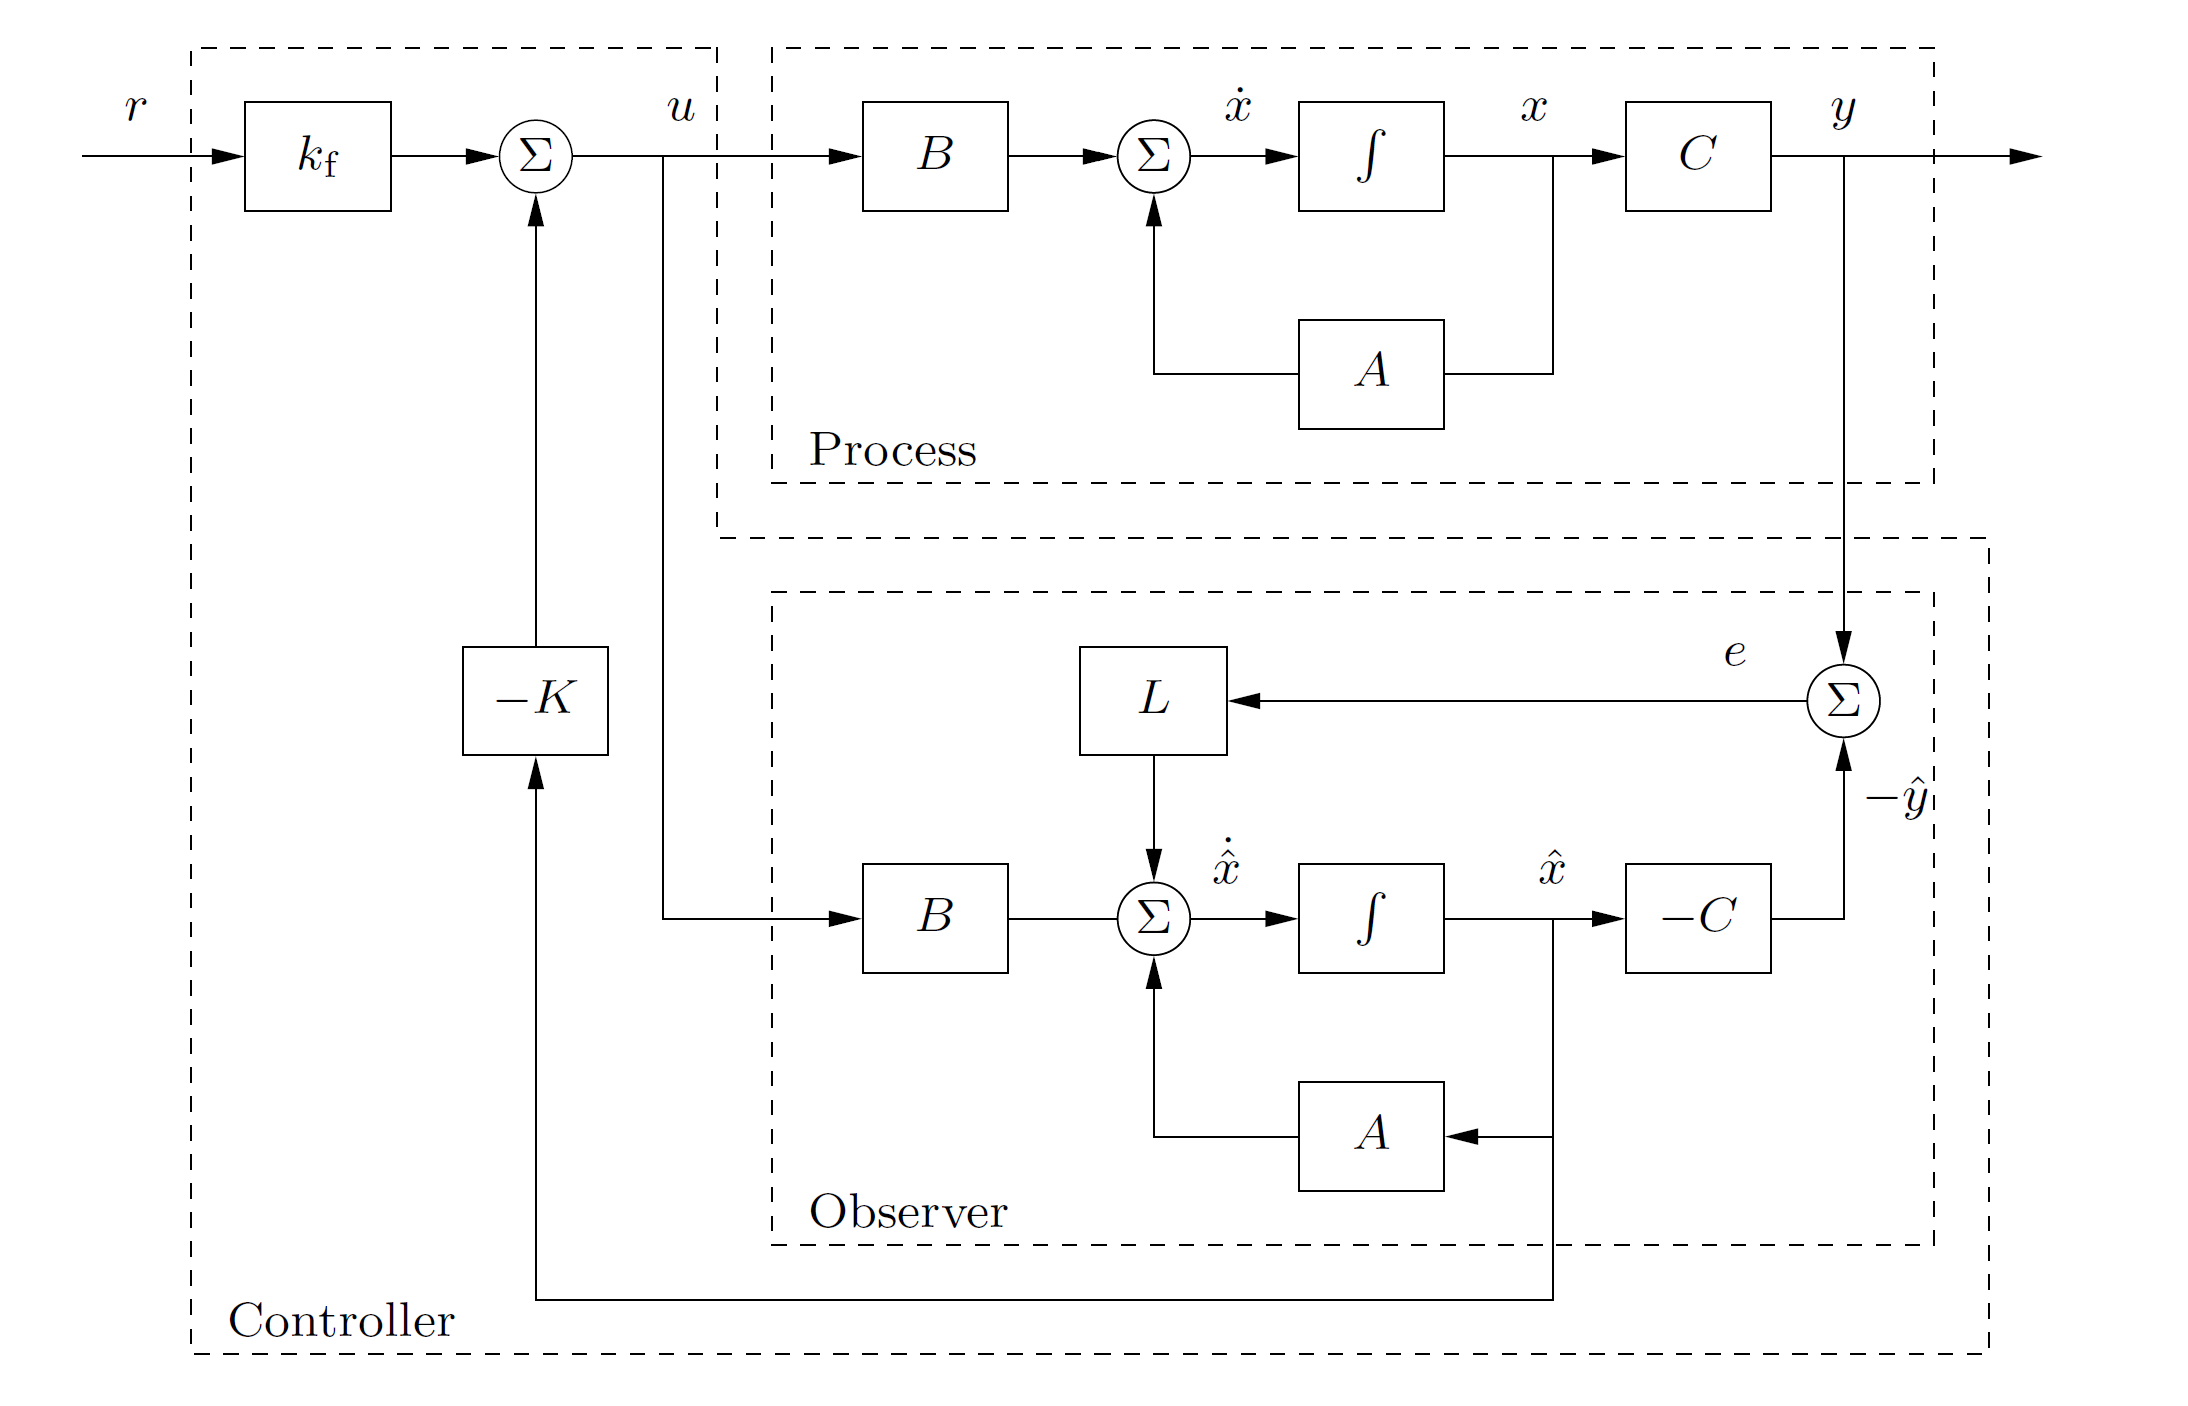
\includegraphics[width = 0.9\textwidth]{outputfeedback.png}  
\end{center}
\end{frame}


\end{document}
